\documentclass[11pt,oneside,a4paper]{book}
\usepackage[spanish]{babel}
\usepackage[latin1]{inputenc}
\usepackage[pdftex]{graphicx}           % para insertar figuras en formato pdf/png/jpg
\usepackage{color}
\usepackage{pifont}
\usepackage{amsfonts}
\usepackage{amssymb} 
\usepackage{setspace}
\usepackage[small,compact]{titlesec}
\usepackage{indentfirst} 
\usepackage[round]{natbib}
\usepackage{subfigure} 	
\usepackage[nottoc]{tocbibind}
\usepackage{setspace}
\usepackage{longtable}
\usepackage{lscape}
\usepackage{caption}
\usepackage{graphicx}
\usepackage{wrapfig}
\usepackage{lscape}
\usepackage{rotating}
\usepackage{epstopdf}
\usepackage[colorlinks=true,urlcolor=red,citecolor=green,linkcolor=blue]{hyperref}
\usepackage[a4paper,top=2.54cm, bottom=2.54cm, left=3cm, right=2.54cm]{geometry} %margenes

% ---------------------------------------------------------------------------- %
\graphicspath{{./figuras/}}
\makeindex  
\raggedbottom
\listfiles
\normalsize

\newcommand{\captionfonts}{\small}
\makeatletter  % Allow the use of @ in command names
\long\def\@makecaption#1#2{%
  \vskip\abovecaptionskip
  \sbox\@tempboxa{{\captionfonts #1: #2}}%
  \ifdim \wd\@tempboxa >\hsize
    {\captionfonts #1: #2\par}
  \else
    \hbox to\hsize{\hfil\box\@tempboxa\hfil}%
  \fi
  \vskip\belowcaptionskip}
\makeatother   % Cancel the effect of \makeatletter

\renewcommand{\topfraction}{0.85}
\renewcommand{\textfraction}{0.1}
\renewcommand{\floatpagefraction}{0.75}

% ---------------------------------------------------------------------------- %
% Cuerpo del texto
\begin{document}
\frontmatter \onehalfspacing

% ---------------------------------------------------------------------------- %
\thispagestyle{empty}
\begin{center}
\vspace*{1cm}
\textbf{\Large{PONTIFICIA UNIVERSIDAD CAT�LICA DEL PER� }}\\
\vspace*{1.2cm}

\textbf{\Large{ESCUELA DE GRADUADOS}}\\
\vspace*{0.5cm}
\begin{center}

\includegraphics[scale=.25]{logoPUCP}
\end{center}
\vspace{0.5cm}

\textbf{\Large{Modelo de censura intervalar\\
  para datos positivos}}\\
\vspace{1.2cm}
\textbf{\large{TESIS PARA OPTAR POR EL GRADO DE MAGISTER EN\\
  ESTAD�STICA}}\\
  
\vspace*{1.2cm}
\textbf{\large{Presentado por:}}\\
\vspace*{0.3cm}
\textbf{\large{Justo Andr�s Manrique Urbina}}\\
\vspace*{1.2cm}
\textbf{\large{Asesor: Cristian Luis Bayes Rodr�guez}}\\

\vspace*{1.2cm}

\textbf{\large{Miembros del jurado:\\
	Dr. Nombre completo jurado 1 \\
	Dr. Nombre completo jurado 2 \\
	Dr. Nombre completo jurado 3  
	}} 
	   
\vspace*{1.2cm}
    
\normalsize{Lima, Diciembre 2020}
\end{center}




%-------------------------------------------
% Dedicatoria
\chapter*{Dedicatoria}
Dedicatoria
%-------------------------------------------



% Agradecimentos
\chapter*{Agradecimentos}
A mi asesor Cristian Bayes y al profesor Giancarlo Sal y Rosas, quienes ofrecieron la 

% ---------------------------------------------------------------------------- %
% Resumen
\chapter*{Resumen}

\noindent \textbf{Palabras clave:} censura intervalar, regresi�n con censura.

% ---------------------------------------------------------------------------- %
% Abstract
\chapter*{Abstract}
Abstract

\noindent \textbf{Keywords:} keyword1, keyword2, keyword3.

% ---------------------------------------------------------------------------- %
% Indice
\tableofcontents    % imprime el indice
% ---------------------------------------------------------------------------- %


\chapter{Lista de Abreviaturas}
\begin{tabular}{ll}
 		fdp     & Funci�n de densidad de probabilidad.\\
	pBF 		& Pseudo factor de Bayes(\emph{Pseudo bayes factor}).\\
\end{tabular}

\chapter{Lista de S�mbolos}
\begin{tabular}{ll}
		$\mu$    & Media.\\
\end{tabular}

\listoffigures               % lista de Figuras
\listoftables                % lista de cuadros

% ---------------------------------------------------------------------------- %
\mainmatter

\onehalfspacing              % interlineado 1.5

%% ------------------------------------------------------------------------- %%
\chapter{Introducci�n}
\label{cap:introduccion}

%% ------------------------------------------------------------------------- %%
Por distintas razones, los datos recabados en una investigaci�n de �ndole estad�stica carecen de precisi�n: existen discrepancias entre el valor real del objeto de medici�n y el valor obtenido. Este proceso puede ser sist�mico: durante la administraci�n de cuestionarios a una poblaci�n objetivo, el encuestado puede omitir, reh�sar o incluso responder incorrectamente preguntas embarazosas o invasivas. Este dilema es conocido entre los encuestadores: sus encuestados, si bien est�n dispuestos a ofrecer la mejor ayuda posible, no est�n dispuestos a ofrecer informaci�n que posteriormente les pueda comprometer. Para obtener dichos datos, el encuestador usa todo su ingenio para equilibrar la privacidad del encuestado y los objetivos de su investigaci�n. En un esfuerzo de aminorar el estr�s del encuestado, el encuestador puede censurar los datos con el fin de obtener una respuesta.

Dichos datos censurados han sido estudiados previamente en la literatura acad�mica. Formalmente, y siguiendo las ideas plasmadas por \cite{peto:p}, una variable $C$ se le denota censurada cuando su valor $c$ no es del todo observable y la �nica informaci�n sobre la misma es un intervalo no-cero $I$. Esta construcci�n permite definir tres tipos de datos censurados: datos censurados \textit{hacia la izquierda} (en d�nde el intervalo $I$ se define de la forma $[-\infty,L_i]$), datos censurados \textit{intervalares} (definido de la forma $[L_i, L_f]; L_i < L_f$), datos censurados \textit{hacia la derecha} (definido de la forma $[L_f, \infty]$). Este tipo de datos naturalmente generan retos en el proceso de modelamiento, pues los modelos est�ndares de regresi�n presumen que la variable respuesta es directamente observable.

Situaciones como la precisada en el parr�fo precedente han sido exploradas previamente: desde la determinaci�n de la verosimilitud, la elaboraci�n de modelos de regresi�n y su estimaci�n bajo inferencia cl�sica y bayesiana. \cite{gentleman:lmk} identificaron un m�todo de m�xima verosimilitud para este tipo de datos, asegurando su consistencia estad�stica e identificando m�todos algor�tmicos para su c�mputo. Utilizado los puntos extremos del intervalo, $L_i$ y $L_f$, era posible identificar la m�xima veros�militud a trav�s de la diferencia de las funciones de distribuci�n acumulada en dichos puntos. Tomando en consideraci�n dicho m�todo de estimaci�n, distintos autores propusieron modelos de regresi�n param�tricos bajo inferencia cl�sica y bayesiana, tales como \cite{mun:xu}, quienes identificaron modelos param�tricos de supervivencia para este tipo de datos.

Cabe resaltar que los modelos anteriormente expuestos identifican el valor esperado de la variable respuesta condicionada por un conjunto de variables. Sin embargo, el inter�s del investigador puede recaer en otro objetivo: m�s all� de la respuesta media, el investigador busca los factores subyacentes que impactan a distintos cuantiles de la variable respuesta. Los factores relacionados a una persona con un gran sueldo son distintos a una persona que no percibe mucho. Para estudios de dicho corte, los modelos de regresi�n cuant�lica brinda la flexibilidad requerida. Dicho modelo fue propuesto inicialmente por Koenker y Basset (1978) quienes, ante la situaci�n en d�nde la estimaci�n de m�nimos cuadrados es deficiente en modelos con errores no gaussianos, proponen una regresi�n de cuantiles que permiten modelar libremente los cuantiles de la variable respuesta en relaci�n a las covariables.

\textbf{Pendiente: Texto explicando los estudios de regresi�n cuant�lica con censura intervalar}

La presente tesis propone utilizar los temas y modelos anteriormente expuestos para implementar un modelo param�trico de regresi�n cuant�lica aplicado a datos con censura intervalar. Para efectos de la aplicaci�n, los datos se modelar�n bajo una distribuci�n Weibull, la cual es de amplia aplicabilidad y permite modelar colas pesadas. Con el prop�sito de implementar la regresi�n cuant�lica y, atendiendo a la estructura de los datos, dicha distribuci�n ser� reparametrizada. Finalmente, el m�todo de estimaci�n ser� el de m�xima verosimilitud, siguiendo el marco de la inferencia cl�sica.

\section{Objetivos}
\label{sec:objetivo}

El objetivo de la tesis consiste en proponer un m�todo de regresi�n cu�ntiliza adaptado a datos con censura intervalar. Para identificar que el modelo propuesto es adecuado, aplicaremos la regresi�n en dos conjuntos de datos: uno simulado y otro real. La base de datos a utilizar ser� la Encuesta Nacional de Satisfacci�n de Usuarios en Salud elaborada por el Instituto Nacional de Estad�stica e Inform�tica el a�o 2015. Los objetivos espec�ficos de la tesis son los siguientes:

\begin{itemize}
	\item Revisar literatura acad�mica relacionada a las propuestas de modelos de regresi�n con datos censurados intervalarmente.
	\item Identificar una estructura apropiada de la distribuci�n Weibull para el modelo de regresi�n cuant�lica v�a una reparametrizaci�n del modelo. Posteriormente, estudiar el comportamiento de dicha estructura.
	\item Estimar los par�metros del modelo propuesto bajo inferencia cl�sica.
	\item Implementar el m�todo de estimaci�n para el modelo propuesto en el lenguaje R y aplicarlo en datos simulados.
	\item Aplicar el modelo propuesto en datos de la Encuesta Nacional de Satisfacci�n de Usuarios en Salud.
\end{itemize}

\section{Organizaci�n del Trabajo}
\label{sec:organizacion}

En el cap�tulo 2, se presenta una estructura de la distribuci�n Weibull, apropiada para los datos con censura intervalar. Por ello, se realiza una parametrizaci�n alternativa y se estudia los 

En el cap�tulo 3, se propone el modelo de regresi�n con datos censurados intervalarmente.

En el cap�tulo 4, se presenta la aplicaci�n del modelo propuesto para determinar si existe diferencia entre los sueldos de enfermeras y enfermeros a lo largo de todos los cuantiles. Ello se realiza mediante inferencia cl�sica.

Finalmente, en el cap�tulo 5 se presentan las principales conclusiones obtenidas en la presente tesis as� como los pr�ximos pasos.

\chapter{Distribuci�n de Weibull}

El presente cap�tulo tiene como objetivo principal proponer una reparametrizaci�n de la distribuci�n de Weibull para adaptarla al modelo de regresi�n cuant�lica. Para dicha reparametrizaci�n, se definir� su funci�n de densidad y funci�n de distribuci�n acumulada, y asimismo se examinar� sus propiedades.

\section{Distribuci�n de Weibull}

La distribuci�n de Weibull fue introducida por \cite{weib:weib}. En dicho art�culo de investigaci�n, Weibull menciona las caracter�sticas de una funci�n de densidad suficientemente flexible para ser adaptada a diversas investigaciones, desde la rama de resistencia de materiales hasta el an�lisis de altura de hombres adultos radicados en las Islas Brit�nicas. Una variable aleatoria continua $Y$, con soporte $Y \in (0,\infty)$, sigue una distribuci�n de Weibull si su funci�n de densidad es dada por la siguiente expresi�n:

\begin{equation}
f{(y)}= \frac{\alpha}{\sigma}\left(\frac{y}{\sigma}\right)^{\alpha-1} \exp{\left(-\frac{y}{\sigma}\right)^{\alpha}}
\end{equation}

\noindent en donde $\alpha > 0$ corresponde al par�metro de forma, y $\sigma > 0$ corresponde al par�metro de escala. La notaci�n de una variable aleatoria $Y$ que sigue esta distribuci�n se indica como $Y \sim W(\alpha,\sigma)$. La funci�n de distribuci�n acumulada de $Y$ tiene la siguiente expresi�n:

\[F{(y)}=1-\exp^{-{(\frac{y}{\sigma})}^{\alpha}}.\]

\noindent Asimismo, su funci�n de cuantiles es dada por:

\[q_{t}=\sigma{(-\log{(1-t)})}^{\frac{1}{\alpha}}\]

\noindent para $0 < t < 1$.

La flexibilidad referida por la distribuci�n de Weibull puede observarse a trav�s de la figura \ref{weib:original}. En dicha figura, observamos que una modificaci�n del par�metro de escala $\sigma$ modifica la tendencia central de la distribuci�n; es decir, se observa que la distribuci�n se mueve en la direcci�n que el par�metro $\sigma$ se mueve. Cabe resaltar que, con un $\alpha$ fijo, la distribuci�n tiende a ser m�s dispersa. Por otro lado, se observa que el aumento del par�metro de forma $\alpha$ contrae la distribuci�n hacia el valor central de la misma. Esto es m�s pronunciado en la medida que dicho par�metro aumenta, manteniendo el par�metro $\sigma$ constante. No obstante, cabe resaltar que la distribuci�n se torna asim�trica en tanto los valores de $\alpha$ son peque�os.

\begin{figure}
	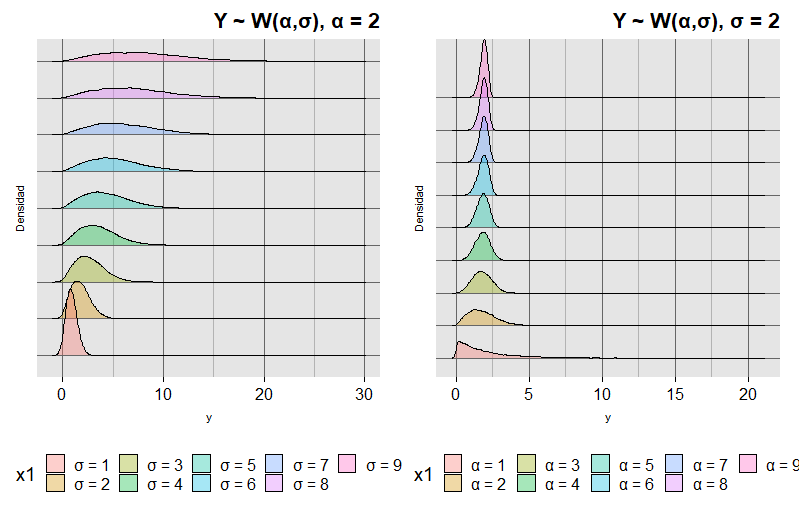
\includegraphics[width=\textwidth]{weib_distrib}
	\caption{Funci�n de densidad de una variable $Y$ con distribuci�n Weibull}
	\label{weib:original}
\end{figure}

Para una variable $Y \sim W(\alpha, \sigma)$, la media y varianza se definen de la siguiente forma:

\[E(Y)=\sigma \Gamma\left( 1+\frac{1}{\alpha} \right).\]
\[V(Y)=\sigma^{2}\left[ \Gamma\left( 1+\frac{2}{\alpha} \right)-\left( \Gamma\left( 1+\frac{1}{\alpha} \right) \right)^{2} \right].\]

\noindent donde $\Gamma(\cdot)$ es la funci�n Gamma.
\section{Hacia una nueva estructura de la distribuci�n de Weibull}
\label{sec2.2}

En esta secci�n consideramos una reparametrizaci�n del par�metro de forma $\sigma$ en t�rminos del cuantil $t, q_{t}$ en los siguientes t�rminos:

\[\sigma = \frac{q_t}{(-\log(1-t))^{\frac{1}{\alpha}}} \]

\noindent en donde $t$ ser� un valor conocido que se encuentra en el intervalo $[0,1]$. Bajo esta nueva estructura, $q_{t}$ y $\alpha$ tienen espacios param�tricos independientes tal que $(q_{t},\alpha) \in (0,\infty) \times (0,\infty)$. Una variable aleatoria $Y$ que sigue una distribuci�n Weibull bajo esta parametrizaci�n se denota como $Y \sim W_{r}(q_{t},\alpha,t)$ y posee la siguiente funci�n de densidad:

\begin{equation}
f_{Y}(y| q_{t},\alpha,t)=\frac{\alpha c(t)}{q_{t}}\left( \frac{y}{q_{t}} \right)^{\alpha-1}\exp\left( -c(t)\left( \frac{y}{q_{t}} \right)^{\alpha} \right)
\end{equation}
\\
\noindent donde $c(t)= \left( -\log(1-t) \right)$. 

Los par�metros $q_{t}$ y $\alpha$, as� como el nivel del cuantil $t$ (el cual es conocido), caracterizan la funci�n de densidad conforme se observa en la Figura \ref{fig:newdens}. En dicha figura, se observa el efecto del nuevo par�metro $q_t$ y el nivel $t$. Podemos observar lo siguiente: 

\begin{itemize}
	\item Se observa que una variaci�n del par�metro $q_t$ conlleva a un aumento en la tendencia central de la distribuci�n hacia la misma direcci�n (en la medida que el par�metro de escala $\alpha$ es constante). Asimismo, para valores bajos de $q_t$, la distribuci�n es leptoc�rtica concolas pronunciadas a la derecha. Asimismo, dicho aumento del par�metro genera valores extremos: la distribuci�n se torna asim�trica, con valores extremos generados cada vez con mayor frecuencia.
	\item Se observa que, para un mismo par�metro $q_t$, la distribuci�n es platic�rtica en la medida que se observe los cuantiles inferiores. Asimismo, en determinados casos pronuncia la asimetr�a identificada anteriormente.
\end{itemize}

\begin{landscape}
\begin{figure}
\centering
	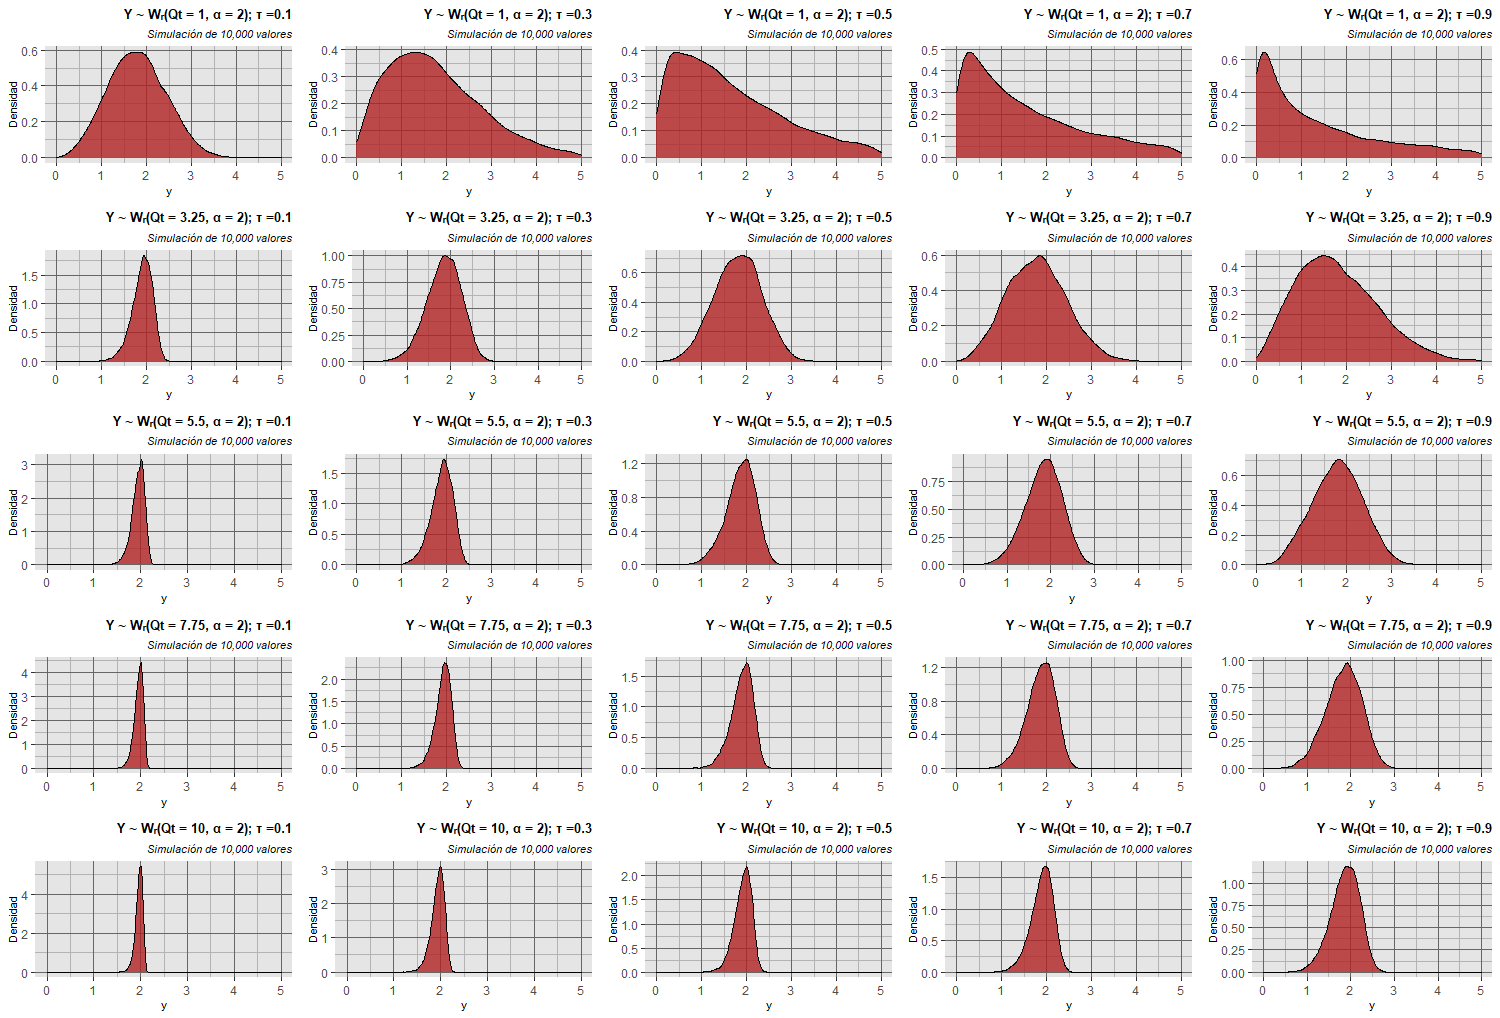
\includegraphics[width=1.5\textheight]{rep_weibull_qt}
	\caption{Densidades de la distribuci�n de Weibull bajo la nueva parametrizaci�n}
	\label{fig:newdens}
\end{figure}
\end{landscape}

\begin{landscape}
	\begin{figure}
		\centering
		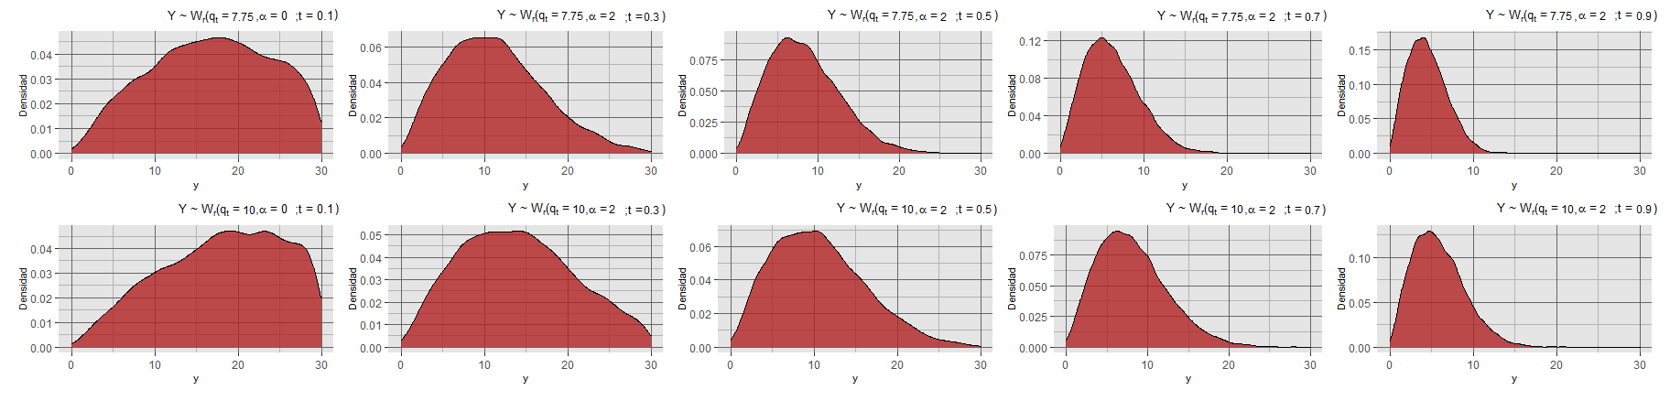
\includegraphics[width=1.5\textheight]{rep_weibull_qt_2}
		\caption{Densidades de la distribuci�n de Weibull bajo la nueva parametrizaci�n}
		\label{fig:newdens2}
	\end{figure}
\end{landscape}

En base a la reparametrizaci�n propuesta, la funci�n de distribuci�n acumulada de $Y \sim W_r(q_t,\alpha,t)$ es de la forma:

\begin{equation} \label{eq:1}
	F_{Y}\left(y| q_{t},\alpha,t \right)=1-\exp\left( -log(1-t)\left( \frac{y}{q_{t}} \right)^{\alpha} \right).
\end{equation}

\noindent Recordemos que $e^{a log(z)} = z^a$, en d�nde $a = -\left(\frac{y}{q_{t}} \right)^{\alpha}$ y $z = (1-t)$. Por lo tanto tenemos:

\begin{equation} \label{eq:2}
F_{Y}\left(y| q_{t},\alpha,t \right)=1-(1-t)^{-\left(\frac{y}{q_{t}} \right)^{\alpha}}.
\end{equation}


Asimismo, el valor esperado y varianza de dicha variable aleatoria est� dada por:

\begin{equation}
E(Y)=\frac{q_{t}}{c(t)^{\frac{1}{\alpha}}}\Gamma\left( 1+\frac{1}{\alpha} \right)
\end{equation}

\begin{equation}
Var(Y)=\frac{q_{t}^{2}}{c(t)^{\frac{1}{\alpha}}}\left[ \Gamma\left( 1+\frac{2}{\alpha}\right)-\Gamma\left( 1+\frac{1}{\alpha} \right)^{2} \right]
\end{equation}

Evaluamos las propiedades de la distribuci�n por cada valor de los par�metros, conforme se observa en la figura \ref{espvar}. Se observa lo siguiente:

\begin{itemize}
	\item \textbf{En relaci�n al valor esperado:}
	\begin{itemize}
		\item Para cada $\alpha$ fijo, el par�metro $q_t$ mueve el valor esperado de la distribuci�n hacia la direcci�n en la que dicho par�metro aumenta o disminuye. Ello se observa a lo largo de todos los posibles valores de $\alpha$. No obstante, la fuerza en que afecta el valor esperado depende del valor de $\alpha$, y se observa que el cambio en la esperanza disminuye en la medida que $\alpha$ aumente.
		\item Para cada $q_t$ fijo, el par�metro $\alpha$ dismuye el valor esperado de la distribuci�n en la medida que dicho par�metro aumente. Este efecto es marginalmente menor por cada aumento de $\alpha$, hasta tener una diferencia m�nima cuando $\alpha$ considere valores cada vez m�s grandes. Asimismo, se observa que la esperanza es alta en la medida que $\alpha$ es peque�o, y esta propiedad aumenta r�pidamente en la medida que $\alpha$ se acerque a 0.
	\end{itemize}
	\item \textbf{En relaci�n a la varianza:}
	\begin{itemize}
		\item De forma similar que en la esperanza, el par�metro $\alpha$ disminuye considerablemente la varianza de la distribuci�n. Esto tiene consistencia con la Figura \ref{weib:original}, pues dicha variable no ha sido reexpresada en t�rminos de la funci�n cuant�lica. Se observa, asimismo, que la varianza es alta en la medida que $\alpha$ es peque�o. Este efecto es mayor cuando el par�metro $q_t$ aumenta conjuntamente.
		\item El par�metro $q_t$ aumenta la varianza de la distribuci�n en la medida este aumente. No obstante, el efecto es modulado por el efecto del par�metro $\alpha$: en la medida que $\alpha$ es alto, el efecto marginal en la varianza por cada aumento de $q_t$ es peque�o. Por otro lado, cuando $\alpha$ es peque�o, el efecto marginal de la varianza por cada aumento de $q_t$ es considerable e incrementa r�pidamente.
	\end{itemize}
\end{itemize}

\begin{figure}
	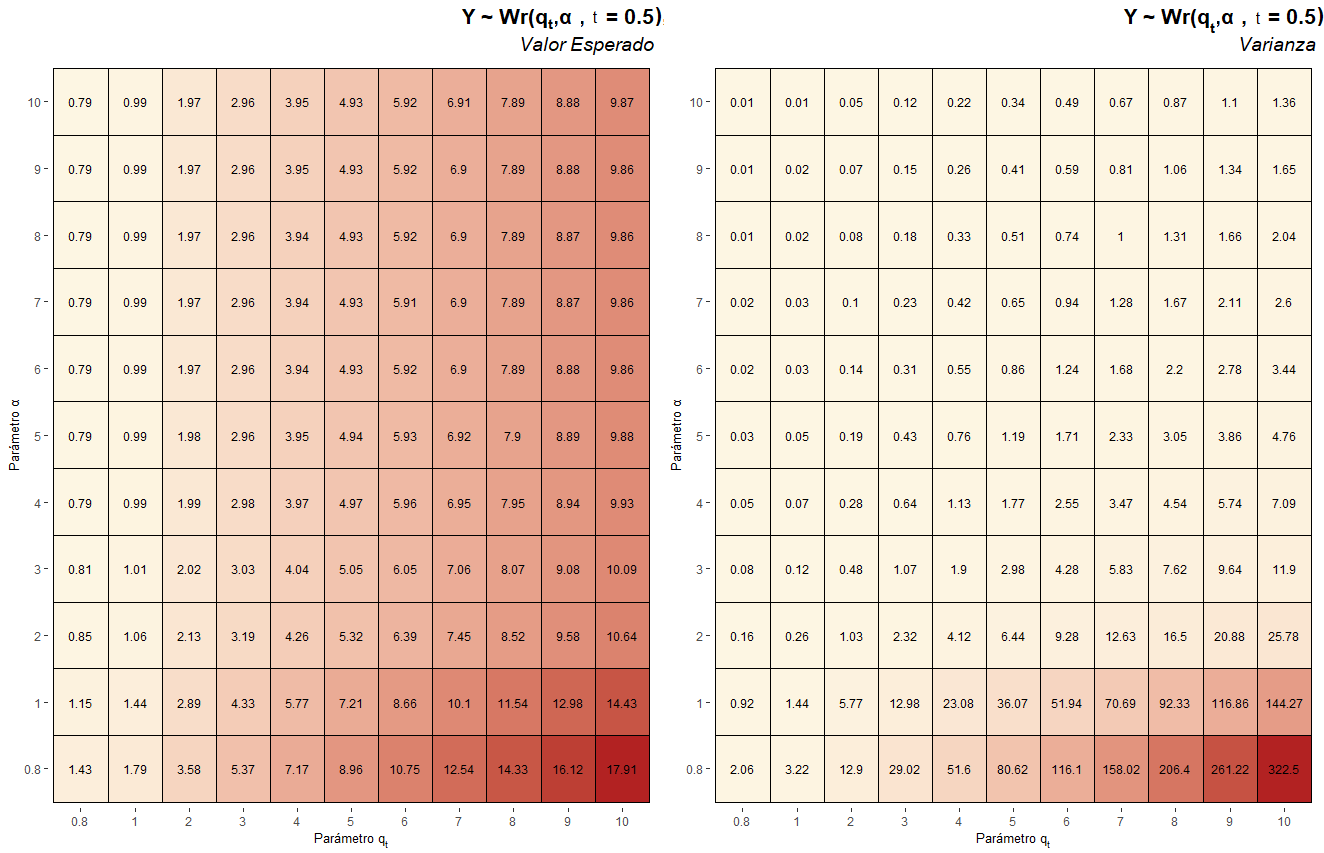
\includegraphics[width=\textwidth]{esperado}
	\caption{Valor esperado y varianza de una distribuci�n Weibull bajo la parametrizaci�n propuesta.}
	\label{espvar}
\end{figure}


\appendix
\chapter{Ap�ndice}

\section{Pseudoc�digo de la simulaci�n}
\label{seudo}

\begin{lstlisting}
Simulamos valores de las siguientes distribuciones:

Definimos los siguientes valores:
N = [100, 500, 1000]
B = [7, 0.3, 0.84, 2.5] 
Sigma = 2
t=[0.1, 0.2, 0.3, 0.4, 0.5, 0.6, 0.7, 0.8, 0.9]
M = 5000

Para cada cuantil en t:
	Para cada n en N:
		Para cada replica en M:
		1 Simular n valores de las siguientes distribuciones:
			X1 ~ Beta(2,3) 
			X2 ~ Normal(2,0.5)
			X3 ~ Gamma(2,25)
		2 Generar la funci�n de enlace:
			Qt = exp(B[1] + B[2]*X1 + B[3]*X2 + B[4]*X3)
		3 Para cada i en n:
			Simular 1 valor de la siguiente distribucion:
			Y[i] ~ W_r(Qt[i], Sigma, cuantil)
		4 Censurar la variable Y de forma intervalar tal que
			Z ~ Categorica
		5 Obtener los limites inferiores y superiores de
			cada categoria de Z
		6 Crear la base de datos simulada
			df <- [L_inf, L_sup, X1, X2, X3]
		7 Ejecutar la regresion de censura intervalar
		8 Guardar los resultados
\end{lstlisting}

\section{Aplicaci�n en R}

\begin{lstlisting}[basicstyle=\tiny]
library(gamlss)
library(gamlss.cens)
library(haven)
library(tidyverse)
library(BB)
library(matrixStats)
library(gridExtra)
library(numDeriv)
library(pracma)
library(ucminf)
library(nloptr)
library(ggthemes)

gen.cens(family="WEI3",type="interval")

Ct = function(alpha, tau){
  (-log(1-tau))^(1/alpha)
}
F_Wr = function(Y,Qt,alpha,tau){
  B = Qt/Ct(alpha,tau)
  pweibull(Y,shape=alpha,scale=B)
}
Qt_b = function(betas, df){
  Qt_c = exp(as.matrix(df[['matriz.diseno']]) %*% betas)
  return(Qt_c)
}
Qt_a = function(betas, df){
  Qt_c = exp(as.matrix(df) %*% betas)
  return(Qt_c)
}
Rand_Wr = function(n,Qt,alpha,tau){
  B = Qt/Ct(alpha,tau)
  rweibull(n,shape = alpha,scale = B)
}
Simulation = function(n){
  X1 = rnorm(n,2,0.25)
  X2 = rbeta(n,2,3)
  X3 = rgamma(n,2,20)
  df = data.frame(X1 = X1, X2 = X2, X3 = X3)
  return(df)
}
DF_Simulation = function(df,betas,alpha,tau){
  M = dim(df)[1]
  design_matrix = model.matrix(~ . ,df)
  Qt_i = Qt_a(betas,design_matrix)
  Y = c()
  for (j in 1:M) {
    Y=rbind(Y,Rand_Wr(1,Qt_i[j],alpha,tau))
  }
  min_Y = floor(min(Y))
  if (min_Y==0) {
    min_Y <- 0.01
  }
  Q8_Y = round(quantile(Y,0.8),2)
  interval = round((Q8_Y-min_Y) / 6,2)
  seq_interv = c(seq(min_Y,Q8_Y,interval),Inf)
  Ls = c()
  for (u in 1:length(Y)) {
    for (n in 1:length(seq_interv)) {
      if (Y[u] <seq_interv[n]) {
        Ls[u] = seq_interv[n]
        break
      }}}
  Li = c()
  for (p in 1:length(Y)) {
    for (w in 1:length(seq_interv)) {
      if (Y[p] > rev(seq_interv)[w]) {
        Li[p] = rev(seq_interv)[w]
        break
      }}}
  F_df = cbind(data.frame(Li = round(Li,2), Ls = round(Ls,2)),df)
  return(F_df)
}
data_mgmt = function(data,li,lf){
  df_inf = data[,li]
  df_sup = data[,lf]
  covar = as.data.frame(data[,-c(li,lf)])
  covar = model.matrix(~. , covar)
  lista = list(lim.inferior = df_inf, lim.superior = df_sup, matriz.diseno = covar)
  return(lista)
}
likelihood = function(param,betas,df,tau){
  n = length(param)-1
  for(i in 1:n){betas[i]=param[i]}
  alpha = param[length(param)]
  Qt_i = Qt_b(betas,df)
  -sum(log(F_Wr(df[['lim.superior']],Qt_i,alpha,tau)
       -F_Wr(df[['lim.inferior']],Qt_i,alpha,tau)))
}
reg_Wr = function(data,li,lf,tau,param){
  df = data_mgmt(data,li,lf)
  Bs = as.matrix(rep(0,ncol(df[['matriz.diseno']])))
  fit_mv = nloptr(x0 = param,eval_f = likelihood, betas=Bs, df=df, tau=tau,
  opts = list("algorithm"=c("NLOPT_LN_SBPLX"),maxeval = 400)
  ,lb = c(-Inf,-Inf,-Inf,-Inf,-Inf,-Inf,-Inf,-Inf,-Inf,-Inf,-Inf)
  ,ub=c(Inf,Inf,Inf,Inf,Inf,Inf,Inf,Inf,Inf,Inf,Inf))
  print(fit_mv$message)
  fit_mv$hessian = pracma::hessian(x0 = fit_mv$solution,f = likelihood,betas=Bs,df=df,tau=tau)
  return(fit_mv)
}

lancet <- function(int){
  temp <- tempfile()
  download.file("http://iinei.inei.gob.pe/iinei/srienaho/descarga/SPSS/447-Modulo552.zip", temp)
  salud <- read_sav(unz(temp, "447-Modulo552/04_C2_CAPITULOS.sav"))
  unlink(temp)
  
  salud <- salud[salud$C2P28 != 7,]
  
  salud$C2P26
  
  ### Pre-procesamiento ###
  variables <- c("INSTITUCION","C2P4","C2P13","C2P21","C2P24","C2P26","C2P28","C2P1","C2P27")
  
  newsalud <- salud[variables]
  
  newsalud$li <- NULL
  newsalud$ls <- NULL
  newsalud$li <- ifelse(newsalud$C2P28 == 1, 850,
                        ifelse(newsalud$C2P28 == 2, 1000,
                               ifelse(newsalud$C2P28 == 3, 2001,
                                      ifelse(newsalud$C2P28 == 4, 3001,
                                             ifelse(newsalud$C2P28 == 5, 4001, 5001)))))
  newsalud$lf <- ifelse(newsalud$C2P28 == 1, 999,
                        ifelse(newsalud$C2P28 == 2, 2000,
                               ifelse(newsalud$C2P28 == 3, 3000,
                                      ifelse(newsalud$C2P28 == 4, 4000,
                                             ifelse(newsalud$C2P28 == 5, 5000, Inf)))))
  
  newsalud <- newsalud %>% select(-C2P28)
  
  newsalud$INSTITUCION <- factor(newsalud$INSTITUCION,labels=names(attr(newsalud$INSTITUCION,"labels")))
  newsalud$C2P4 <- factor(newsalud$C2P4,labels = names(attr(newsalud$C2P4,"labels")))
  newsalud$C2P13 <- factor(newsalud$C2P13, labels=names(attr(newsalud$C2P13,"labels")))
  newsalud$C2P21 <- as.integer(newsalud$C2P21)
  newsalud$C2P24 <- factor(newsalud$C2P24, labels = names(attr(newsalud$C2P24,"labels")))
  newsalud$C2P26 <- factor(newsalud$C2P26, labels = names(attr(newsalud$C2P26,"labels")))
  newsalud$C2P1 <- factor(newsalud$C2P1, labels = names(attr(newsalud$C2P1,"labels")))
  newsalud$C2P27 <- as.integer(newsalud$C2P27)
  
  newsalud_enf <- newsalud[newsalud$C2P1 =="Enfermero/a" ,]
  newsalud_enf <- subset(newsalud_enf, select = -C2P1)
  newsalud_enf <- as.data.frame(newsalud_enf)
  
  newsalud_med <- newsalud[newsalud$C2P1 == "M�dico",]
  newsalud_med <- subset(newsalud_med, select = -C2P1)
  newsalud_med <- as.data.frame(newsalud_med)
  if (int == 1) {
    return(newsalud_enf)  
  }
  if (int ==2) {
    return(newsalud_med)
  }
  if (int ==3) {
    newsalud_total <- as.data.frame(subset(newsalud,select = -C2P1))
    return(newsalud_total)
  }
}

#### Simulaci�n ####

L = 5000
n = c(100,500,1000)
betas_sim = c(7,0.3,0.84,2.5)
alpha_sim = 2
tau_sim = seq(0.1,0.9,0.1)

sim_list= list(n100 = list(), n500 = list(), n1000 = list())

for (j in 1:length(n)) {
  for (k in 1:length(tau_sim)) {
    for (p in 1:L) {
      sim = Simulation(n[j])
      df_sim = DF_Simulation(sim,betas_sim,alpha_sim,tau_sim[k])
      m0 = gamlss(Surv(Li,Ls,type="interval2")~.,family = WEI3ic,data = na.omit(df_sim))
      init = as.vector(c(coef(m0),m0$sigma.coefficients))
      sim_list[[j]] = append(sim_list[[j]],list(reg_Wr(data = df_sim,
                       li = 1,lf = 2,tau = tau_sim[k],param = init)))
    }
  }
}

se_calc <- function(lista) {
  ic_contain <- matrix(nrow=0,ncol=5)
  for (k in 1:length(lista)) {
    little_t <- lista[[k]]
    ic <- rbind( little_t$par - qnorm(0.975) * sqrt(diag(solve(little_t$hessian))),
                 little_t$par + qnorm(0.975) * sqrt(diag(solve(little_t$hessian))))
    ic_contain <- rbind(ic_contain,cbind(between(betas_sim[1],left = ic[1,1],right = ic[2,1]),
                        between(betas_sim[2],left = ic[1,2],right = ic[2,2]),
                        between(betas_sim[3],left = ic[1,3],right = ic[2,3]),
                        between(betas_sim[4],left = ic[1,4],right = ic[2,4]),
                        between(alpha_sim,left = ic[1,5],right = ic[2,5])))
  }
  final_df <- as.matrix(t(colSums(ic_contain)/length(lista)))
  return(final_df)
}

final_database <- matrix(nrow=0,ncol=5)
seq_t <- seq(1,8,1);seq_t

for (j in 1:length(n)) {
  df <- sim_list[[j]]
  actual_t <- df[1:5000*seq_t[1]]
  vf_df <- se_calc(actual_t)
  rownames(vf_df) <- paste("n_",n[j],sep="")
  final_database <- rbind(final_database,vf_df)
  
  for (l in 1:length(seq_t)) {
   actual_t <-  df[(5000*seq_t[l]+1):(5000*(seq_t[l]+1))]
   vf_df <- se_calc(actual_t)
   rownames(vf_df) <- paste("n_",n[j],sep="")
   final_database <- rbind(final_database,vf_df)
  }
}

final_database <- as.data.frame(final_database)

final_database_vf <- cbind(
  Cuantil = rep(c('0.1','0.2','0.3','0.4','0.5','0.6','0.7','0.8','0.9'),3),
  B1 = c(rep(100,9),rep(500,9),rep(1000,9)), 
  final_database)

v1 <- ggplot(data = final_database_vf) +
  aes(x = "", y = V1) +
  geom_boxplot(shape = "circle", fill = "#B22222") +
  facet_wrap(vars(B1)) +
  scale_color_brewer(palette = "YlOrRd") + 
  labs(x="Tama�o de Muestra", y="Cobertura",title = "Cobertura para \U003B2_0") +
  scale_y_continuous(limits=c(0.93,0.96)) + 
  geom_hline(yintercept=0.95,linetype="dashed",color="red")+
  theme_minimal() +
  theme(legend.position="bottom")

v2 <- ggplot(data = final_database_vf) +
  aes(x = "", y = V2) +
  geom_boxplot(shape = "circle", fill = "#B22222") +
  facet_wrap(vars(B1)) +
  scale_color_brewer(palette = "YlOrRd") + 
  labs(x="Tama�o de Muestra", y="Cobertura",title = "Cobertura para \U003B2_1") +
  scale_y_continuous(limits=c(0.93,0.96)) + 
  geom_hline(yintercept=0.95,linetype="dashed",color="red")+
  theme_minimal() +
  theme(legend.position="bottom")

v3 <- ggplot(data = final_database_vf) +
  aes(x = "", y = V3) +
  geom_boxplot(shape = "circle", fill = "#B22222") +
  facet_wrap(vars(B1)) +
  scale_color_brewer(palette = "YlOrRd") + 
  labs(x="Tama�o de Muestra", y="Cobertura",title = "Cobertura para \U003B2_2") +
  scale_y_continuous(limits=c(0.93,0.96)) + 
  geom_hline(yintercept=0.95,linetype="dashed",color="red")+
  theme_minimal() +
  theme(legend.position="bottom")

v4 <- ggplot(data = final_database_vf) +
  aes(x = "", y = V4) +
  geom_boxplot(shape = "circle", fill = "#B22222") +
  facet_wrap(vars(B1)) +
  scale_color_brewer(palette = "YlOrRd") + 
  labs(x="Tama�o de Muestra", y="Cobertura",title = "Cobertura para \U003B2_3") +
  scale_y_continuous(limits=c(0.93,0.96)) + 
  geom_hline(yintercept=0.95,linetype="dashed",color="red")+
  theme_minimal() +
  theme(legend.position="bottom")

v5 <- ggplot(data = final_database_vf) +
  aes(x = "", y = V5) +
  geom_boxplot(shape = "circle", fill = "#B22222") +
  facet_wrap(vars(B1)) +
  scale_color_brewer(palette = "YlOrRd") + 
  labs(x="Tama�o de Muestra", y="Cobertura",title = "Cobertura para \U003B1") +
  scale_y_continuous(limits=c(0.93,0.96)) + 
  geom_hline(yintercept=0.95,linetype="dashed",color="red")+
  theme_minimal() +
  theme(legend.position="bottom")

ggpubr::ggarrange(v1,v2,v3,v4,v5)

ecm_calc <- function(lista) {
  ic_contain <- matrix(nrow=0,ncol=5)
  for (k in 1:length(lista)) {
    little_t <- lista[[k]]
    ecm <- (little_t$par - c(betas_sim,alpha_sim))**2
    ic_contain <- rbind(ic_contain,ecm)
  }
  final_df <- as.matrix(t(colSums(ic_contain)/length(lista)))
  return(final_df)
}

  final_database <- matrix(nrow=0,ncol=5)

seq_t <- seq(1,8,1);seq_t

for (j in 1:length(n)) {
  df <- sim_list[[j]]
  actual_t <- df[1:5000*seq_t[1]]
  vf_df <- ecm_calc(actual_t)
  rownames(vf_df) <- paste("n_",n[j],sep="")
  final_database <- rbind(final_database,vf_df)
  
  for (l in 1:length(seq_t)) {
    actual_t <-  df[(5000*seq_t[l]+1):(5000*(seq_t[l]+1))]
    vf_df <- ecm_calc(actual_t)
    rownames(vf_df) <- paste("n_",n[j],sep="")
    final_database <- rbind(final_database,vf_df)
  }
}
round(final_database,4)

final_database <- as.data.frame(final_database)

final_database_vf <- cbind(
  Cuantil = rep(c('0.1','0.2','0.3','0.4','0.5','0.6','0.7','0.8','0.9'),3),
  B1 = c(rep(100,9),rep(500,9),rep(1000,9)), 
  final_database)

v1 <- ggplot(data = final_database_vf) +
  geom_line(aes(x=B1,y=V1,color=Cuantil,group=Cuantil),size=1.2) +
  scale_color_brewer(palette = "YlOrRd") + 
  labs(x="Tama�o de Muestra", y="ECM",title = "ECM para \U003B2_0") +
  scale_x_continuous(breaks=c(100,500,1000)) +
  theme_minimal() +
  theme(legend.position="bottom")


v2 <- ggplot(data = final_database_vf) +
  geom_line(aes(x=B1,y=V2,color=Cuantil,group=Cuantil),size=1.2) +
  scale_color_brewer(palette = "YlOrRd") + 
  labs(x="Tama�o de Muestra", y="ECM",title = "ECM para \U003B2_1") +
  scale_x_continuous(breaks=c(100,500,1000)) + 
  theme_minimal() +
  theme(legend.position="bottom")

v3 <- ggplot(data = final_database_vf) +
  geom_line(aes(x=B1,y=V3,color=Cuantil,group=Cuantil),size=1.2) +
  scale_color_brewer(palette = "YlOrRd") + 
  labs(x="Tama�o de Muestra", y="ECM",title = "ECM para \U003B2_2") +
  scale_x_continuous(breaks=c(100,500,1000)) + 
  theme_minimal() +
  theme(legend.position="bottom")

v4 <- ggplot(data = final_database_vf) +
  geom_line(aes(x=B1,y=V4,color=Cuantil,group=Cuantil),size=1.2) +
  scale_color_brewer(palette = "YlOrRd") + 
  labs(x="Tama�o de Muestra", y="ECM",title = "ECM para \U003B2_3") +
  scale_x_continuous(breaks=c(100,500,1000)) + 
  theme_minimal() +
  theme(legend.position="bottom")

v5 <- ggplot(data = final_database_vf) +
  geom_line(aes(x=B1,y=V5,color=Cuantil,group=Cuantil),size=1.2) +
  scale_color_brewer(palette = "YlOrRd") + 
  labs(x="Tama�o de Muestra", y="ECM",title = "ECM para \U003B1") +
  scale_x_continuous(breaks=c(100,500,1000)) + 
  theme_minimal() +
  theme(legend.position="bottom")

ggpubr::ggarrange(v1,v2,v3,v4,v5)

ses_calc <- function(lista) {
  ic_contain <- matrix(nrow=0,ncol=5)
  for (k in 1:length(lista)) {
    little_t <- lista[[k]]
    ecm <- (little_t$par - c(betas_sim,alpha_sim))
    ic_contain <- rbind(ic_contain,ecm)
  }
  final_df <- as.matrix(t(colSums(ic_contain)/length(lista)))
  return(final_df)
}

final_database <- matrix(nrow=0,ncol=5)

seq_t <- seq(1,8,1);seq_t

for (j in 1:length(n)) {
  df <- sim_list[[j]]
  actual_t <- df[1:5000*seq_t[1]]
  vf_df <- ses_calc(actual_t)
  rownames(vf_df) <- paste("n_",n[j],sep="")
  final_database <- rbind(final_database,vf_df)
  
  for (l in 1:length(seq_t)) {
    actual_t <-  df[(5000*seq_t[l]+1):(5000*(seq_t[l]+1))]
    vf_df <- ses_calc(actual_t)
    rownames(vf_df) <- paste("n_",n[j],sep="")
    final_database <- rbind(final_database,vf_df)
  }
}

final_database <- as.data.frame(final_database)

final_database_vf <- cbind(
  Cuantil = rep(c('0.1','0.2','0.3','0.4','0.5','0.6','0.7','0.8','0.9'),3),
  B1 = c(rep(100,9),rep(500,9),rep(1000,9)), 
  final_database)

v1 <- ggplot(data = final_database_vf) +
  aes(x = "", y = V1) +
  geom_boxplot(shape = "circle", fill = "#EF562D") +
  facet_grid(vars(), vars(B1)) +
  scale_color_brewer(palette = "YlOrRd") + 
  labs(x="Tama�o de Muestra", y="Sesgo Relativo",title = "Sesgo Relativo para \U003B2_0") +
  geom_hline(yintercept=0.0,linetype="dashed",color="black") +
  scale_y_continuous(limits=c(-0.025,0.025)) +
  theme_minimal() +
  theme(legend.position="bottom")

v2 <- ggplot(data = final_database_vf) +
  aes(x = "", y = V1) +
  geom_boxplot(shape = "circle", fill = "#EF562D") +
  facet_grid(vars(), vars(B1)) +
  scale_color_brewer(palette = "YlOrRd") + 
  labs(x="Tama�o de Muestra", y="Sesgo Relativo",title = "Sesgo Relativo para \U003B2_1") +
  geom_hline(yintercept=0.0,linetype="dashed",color="black") +
  scale_y_continuous(limits=c(-0.025,0.025)) +
  theme_minimal() +
  theme(legend.position="bottom")

v3 <- ggplot(data = final_database_vf) +
  aes(x = "", y = V1) +
  geom_boxplot(shape = "circle", fill = "#EF562D") +
  facet_grid(vars(), vars(B1)) +
  scale_color_brewer(palette = "YlOrRd") + 
  labs(x="Tama�o de Muestra", y="Sesgo Relativo",title = "Sesgo Relativo para \U003B2_2") +
  geom_hline(yintercept=0.0,linetype="dashed",color="black") +
  scale_y_continuous(limits=c(-0.025,0.025)) +
  theme_minimal() +
  theme(legend.position="bottom")

v4 <- ggplot(data = final_database_vf) +
  aes(x = "", y = V1) +
  geom_boxplot(shape = "circle", fill = "#EF562D") +
  facet_grid(vars(), vars(B1)) +
  scale_color_brewer(palette = "YlOrRd") + 
  labs(x="Tama�o de Muestra", y="Sesgo Relativo",title = "Sesgo Relativo para \U003B2_3") +
  geom_hline(yintercept=0.0,linetype="dashed",color="black") +
  scale_y_continuous(limits=c(-0.025,0.025)) +
  theme_minimal() +
  theme(legend.position="bottom")

v5 <- ggplot(data = final_database_vf) +
  aes(x = "", y = V1) +
  geom_boxplot(shape = "circle", fill = "#EF562D") +
  facet_grid(vars(), vars(B1)) +
  scale_color_brewer(palette = "YlOrRd") + 
  labs(x="Tama�o de Muestra", y="Sesgo Relativo",title = "Sesgo Relativo para \U003B1") +
  geom_hline(yintercept=0.0,linetype="dashed",color="black") +
  theme_minimal() +
  theme(legend.position="bottom")

ggpubr::ggarrange(v1,v2,v3,v4,v5)

#### Datos reales ####

real_data_enf = lancet(3)
real_data_med = real_data_enf

library(skimr)

enf <- real_data_med %>% mutate(factor = case_when(lf == 999 ~ 1, lf == 2000 ~ 2, lf == 3000 ~ 3, lf == 4000 ~ 4,lf == 5000 ~ 5, lf == Inf ~ 6))
enf$factor <- factor(x = enf$factor,labels = c("[850-999]","[1000-2000]","[2001-3000]","[3001-4000]","[4001-5000]","[5001-Inf.]"))

ib <- enf %>% group_by(factor) %>% skim()

enf %>% group_by(factor,INSTITUCION) %>% summarise( n())



tau_seq_sim = seq(0.1,0.90,0.1)
#m1 = gamlss(Surv(li,lf,type="interval2")~.,family = WEI3ic,data = real_data_enf)
m2 = gamlss(Surv(li,lf,type="interval2")~.,family = WEI3ic,data = real_data_med)
# init_real_enf = as.vector(c(coef(m1),m1$sigma.coefficients))
init_real_med = as.vector(c(coef(m2),exp(m2$sigma.coefficients)))
abc <- confint(m2)
#### Regresi�n cuant�lica para m�dicxs ####

var_med = list()
for (j in 1:length(tau_seq_sim)) {
  var_med = append(var_med,list(reg_Wr(data = real_data_med,li = 8, lf = 9,tau_seq_sim[j],param = init_real_med)))
}

col_df <- c(colnames(model.matrix( ~ . ,subset.data.frame(real_data_med,select = -c(8,9)))),"\U03B1")
val_med <- matrix(ncol=8,nrow = 0)

for (l in 1:length(tau_seq_sim)) {
  pba <- var_med[[l]]
  val_med <- rbind(val_med,
                   cbind(pba$solution,
                         col_df,
                         tau_seq_sim[l],
                         init_real_med,
                         pba$solution + qnorm(0.975) * sqrt(diag(solve(pba$hessian))),
                         pba$solution - qnorm(0.975) * sqrt(diag(solve(pba$hessian))),
                         c(abc[,1],exp(m2$sigma.coefficients)),
                         c(abc[,2],exp(m2$sigma.coefficients))
                         ))
}
val_med <- as.data.frame(val_med)
val_med$V1 <- exp(as.numeric(val_med$V1))
val_med$V3 <- as.numeric(val_med$V3)
val_med$V5 <- exp(as.numeric(val_med$V5))
val_med$V6 <- exp(as.numeric(val_med$V6))
val_med$V7 <- exp(as.numeric(val_med$V7))
val_med$V8 <- exp(as.numeric(val_med$V8))
val_med$init_real_med <- as.numeric(val_med$init_real_med)


ggplot(val_med) +
  aes(x = V3, y = V1) +
  geom_ribbon(mapping = aes(ymin = V6,ymax = V5),fill = "#B2B9FF") +
  geom_line(size = 0.5, colour = "#1B00FF") +
  geom_ribbon(mapping = aes(ymin = V7,ymax = V8),fill = "#cccccc",alpha=0.5) +
  geom_line(mapping = aes(y=exp(init_real_med)),size=0.5) + 
  ggthemes::theme_pander() +
  facet_wrap(vars(col_df), scales = "free")

\end{lstlisting}
      % associado ao arquivo: 'ape-1.tex'

% ---------------------------------------------------------------------------- %
% Bibliografia
\backmatter \singlespacing   % espacio simple

\renewcommand{\harvardand}{y} % cambiar "and" por "y" al generar la bibliografia.
\bibliography{bibliografia}
\bibliographystyle{dcu}

\end{document}
